\documentclass[11pt, english]{article}
        \usepackage{geometry}
                \geometry{
                        a4paper,total={210mm,297mm},
                        tmargin=36mm,
                        bmargin=36mm,
                        lmargin=30mm,
                        rmargin=30mm,
                }

	\usepackage{titlesec}
                \titleformat{\section}
                        {\normalfont\fontsize{18}{16}\bfseries}{\thesection}{0.5em}{}
                \titleformat{\subsection}
                        {\normalfont\fontsize{14}{16}\bfseries}{\thesubsection}{1em}{}
                \titleformat{\subsubsection}
                        {\normalfont\fontsize{11}{16}\bfseries}{\thesubsubsection}{1em}{}

	\usepackage{float}

	\usepackage{longtable}
        \usepackage{multirow}

	\usepackage{caption}
                \captionsetup[table]{labelfont=bf,textfont=bf,font=small,skip=8pt}
                \captionsetup[figure]{labelfont=bf,textfont=bf,font=small,skip=8pt}
        \usepackage{subcaption}
                \captionsetup[subtable]{labelfont=rm,textfont=rm,font=small,skip=8pt,labelformat=parens,labelsep=space}
                \captionsetup[subfigure]{labelfont=rm,textfont=rm,font=small,skip=8pt,labelformat=parens,labelsep=space}

	\renewcommand{\thetable}
                {\thesection.\arabic{table}}                                                         
	\renewcommand{\thesubtable}
                {\roman{subtable}}

	\renewcommand{\thefigure}
                {\thesection.\arabic{figure}}
        \renewcommand{\thesubfigure}
                {\roman{subfigure}}

        \usepackage{hyperref}
                \hypersetup{
                        colorlinks=true,
                        linkcolor=black,
                        filecolor=magenta,
                        urlcolor=cyan,
                        }

        \setlength{\parindent}{0pt}
        \renewcommand{\baselinestretch}{1.25}
        \usepackage{setspace}

        \usepackage{amsmath}
        \usepackage{amssymb}

	\usepackage{graphicx}

	\usepackage[utf8]{inputenc}
	\usepackage[T1]{fontenc}

\begin{document}

\pagenumbering{gobble}

	\title{\textsc{CS991 Mobile Application Development\\ Coursework Assignment}}
	\author{\textsc{Lewis Britton}}
	\date{\textsc{Academic Year 2021/2022}}
        \maketitle

\newpage

\pagenumbering{roman}

	\renewcommand{\contentsname}{Table of Contents}

	\tableofcontents

\newpage

\pagenumbering{arabic}

\section*{The Task}

	\subsection*{Overview}

	\begin{enumerate}
	\setlength\itemsep{0cm}
		\item \textit{Usability} evaluation techniques
		\item Graphical User Interface on \textit{protoyping} level
		\item \textit{Requirements} analysis
		\item Role of either: \textit{developer} or \textit{software engineer}
	\end{enumerate}

	\subsection*{Target}

	\begin{itemize}
	\setlength\itemsep{0cm}
		\item Students
		\item Course directors
	\end{itemize}

	\subsection*{Specification}

	\textit{CIS Personal Circumstances Manager} which [1] allows (registered) students to record personal circumstances and [2] allows course directors to monitor the personal circumstances of students during the academic year.

	\begin{itemize}
	\setlength\itemsep{0cm}
		\item Students
		\begin{itemize}
			\item Log in to institution w/ username and password
			\item View current and historic personal cicumstances
			\item Edit current personal circumstances
			\item Delete current personal circumstances
			\item Add new personal circumstances (start date, end date, description, optional attachment w/ evidence)
			\item Log out
		\end{itemize}
		\item Course Directors
		\begin{itemize}
			\item Log in to institution w/ username and password
			\item View list of students w/ recorded personal circumstances
			\item View details of each personal circumstances entry
			\item Search for student using registration number
			\item Order personal circumstances by start date - most recent
			\item Log out
		\end{itemize}
	\end{itemize}	

\newpage

\section{Core Task: Heuristic Evaluation}

	\subsection{Basics}

	As an alternative to empirical, formal and automated methodologies where people or a series of pre-defined simulations test software throughout various stages and levels of relevance in the design process; Nielsen (1994) proposes a critique-based heuristic evaluation method which involves feedback relative to particular areas of expertise. Niesel finds that this approach is effective before user testing, as minor issues should not be allocated space or time in user testing; before redesign, as relevant subjective opinion may skew in a direction not necessarily followed initially; when you're aware of issues however desire assurance so time is not wasted on them; and, pre-final release for the final polish.\\

	Nielsen also claims that the optimal number of `experts' assigned to an evaluation is three to five, in order to find the optimal number of problems relative to the cost-benefit analysis. In this case however, of course only one is being used as the problem sample is likely to be extremely small. Each problem should be listed indivdually and marked against the set of ten heuristic factors and a severity rating, as seen in Table 1.1. There should be two or three passes upon each problem.\\

	\begin{table}[h]
		\scriptsize
		\renewcommand{\arraystretch}{1.25}
	\begin{center}
	\begin{tabular}{c}
		\hline
		Heuristics\\
		\hline
		\multicolumn{1}{l}{$\mathrm{H_{1}}$: Visibility of System Status}\\
		\multicolumn{1}{l}{$\mathrm{H_{2}}$: System-Real-World Match}\\
		\multicolumn{1}{l}{$\mathrm{H_{3}}$: User Control \& Freedom}\\
		\multicolumn{1}{l}{$\mathrm{H_{4}}$: Consistency \& Standards}\\
		\multicolumn{1}{l}{$\mathrm{H_{5}}$: Error Prevention}\\
		\multicolumn{1}{l}{$\mathrm{H_{6}}$: Recognition Rather than Recall}\\
		\multicolumn{1}{l}{$\mathrm{H_{7}}$: Flexibility \& Efficiency of Use}\\
		\multicolumn{1}{l}{$\mathrm{H_{8}}$: Aesthetic \& Minimalist Design}\\
		\multicolumn{1}{l}{$\mathrm{H_{9}}$: User Recognition, Diagnostic \& Recovery from Error}\\
		\multicolumn{1}{l}{$\mathrm{H_{10}}$: Help \& Documentation}\\
		\hline
		Severity Ratings\\
		\hline
		\multicolumn{1}{l}{$\mathrm{S_{0}}$: Don't think it is a usability problem}\\
		\multicolumn{1}{l}{$\mathrm{S_{1}}$: Cosmetic issue; repair in additional time}\\
		\multicolumn{1}{l}{$\mathrm{S_{2}}$: Minor usability problem; allocate low priority to repair}\\
		\multicolumn{1}{l}{$\mathrm{S_{3}}$: Major usability problem; allocate high priority to repair}\\
		\multicolumn{1}{l}{$\mathrm{S_{4}}$: Critical error; repair immediately}\\
		\hline
	\end{tabular}
		\caption{Heuristics \& Severity Rating}
	\end{center}
	\end{table}

\newpage

	\subsection{Analysis}

	\begin{center}
		\scriptsize
	\begin{longtable}{p{7.5cm}p{0.5cm}p{0.5cm}p{4cm}}
		\textsc{Description} & \textsc{Vio.} & \textsc{Sev.} & \textsc{Proposed Solution}\\
		\hline
		\textbf{Location}:\newline Adding a personal circumstances report is a very common protocol amongst students, from my experience. Although I've never completed one myself, at least (approx.) 30\% of students I've known have. Therefore, that makes this feature just as relevant as something like booking a library room, for example. Which is a prominant feature. This feature should be just as accessible. & $\mathrm{H_{7}}$ & $\mathrm{S_{2}}$ & Create major link as opposed to hierarchical path.\\
		\textbf{Spacing}:\newline Major heading on the primary form page has inconsistent spacing (margins/ local padding) which is too small and looks improper against the consistently high line height throughout the form. & $\mathrm{H_{4}}$, $\mathrm{H_{8}}$ & $\mathrm{S_{1}}$ & Increase heading margin.\\
		\textbf{Scaling}:\newline Page does not scale well to medium--small device widths. This means elements are lost and unreadable & $\mathrm{H_{8}}$ & $\mathrm{S_{1}}$ & Correct style scaling to scale below 300\%.\\
		\textbf{Gutters}:\newline White space gutters in main text body division appear too narrow and therefore make long strings of text harder to read. This also makes elements such as the text input box appear to wide. & $\mathrm{H_{8}}$ & $\mathrm{S_{1}}$ & Increase gutters by approximately 5\%\\
		\textbf{Date Input Boxes}:\newline Input boxes for `first date of circumstance' and `last date of circumstance' are of \verb|text| type and therefore there is a greyscale prompt posted above the input boxes to encourage the user to follow a particular format, which is just awkward as users must enter a series of special characters in particular places. & $\mathrm{H_{7}}$ & $\mathrm{S_{2}}$ & Change the input type of the input boxes to date so there is always the correctly defined input format, and remove the greyscale prompt.\\
		\textbf{Date Select}:\newline Next to the input boxes for the discussed dates, are optional date select features which allow the user to find dates using a calendar system. These features open in a new browser window. This may be an issue where certain user browser preferences may block features such as links opening new windows, etc. The user may also be left unaware of what the issue is if the new window does not open as there is no protocol in place to inform them. & $\mathrm{H_{3}}$, $\mathrm{H_{4}}$, $\mathrm{H_{5}}$ & $\mathrm{S_{2}}$ & By inlcluding these date select features as a drop-down or pop-up overlay would reduce browser associated issues. Further, removing the feature all-together may be more effective in reducing bloat, if the previously discussed amendments to the date input boxes are implemented.\\
		\textbf{Date Select Window}:\newline The graphic design/styling of the new window displaying the date select calendar is completely inconsistent with the primary Pegasus stylesheet. This isn't really a big issue as your just selecting three things however, for the sake of consistency and continuity, this is inappropriate. & $\mathrm{H_{4}}$, $\mathrm{H_{8}}$ & $\mathrm{S_{2}}$ & Amend, for consistency: colors: spacing, font, font-decoration, margin and padding standards, table borders, to name a few.\\
		\textbf{Description Input Box}:\newline The description input box has an infinite character limit but a text prompt and subsequent example encouraging the user to keep their text brief. This is bloated and ineffective as the user is still free to abuse the input box. Additionally, the prompt and example take up space with, effectively irrelevant, content which can be replaced with additional minor functionality features. & $\mathrm{H_{1}}$ (Space), $\mathrm{H_{7}}$, $\mathrm{H_{8}}$ & $\mathrm{S_{2}}$ & Include a word limit and placeholder which restricts and prompts the user to keep their text brief in a more effective manner.\\
		\textbf{Edit Practicality}:\newline If a user wishes to alter an existing personal circumstances request, they are prompted to enter their active requests, delete the one with an error and create a new one in its place. This is unecessarily time consuming for the user. & $\mathrm{H_{5}}$, $\mathrm{H_{7}}$ & $\mathrm{S_{2}}$ & Add a feature which allows users to edit the 3 input elements (start date, end date and description) of their existing requests.\\
		\textbf{Session Time-Out}:\newline A more general issue with Pegasus; there is no prompt to allow the user to choose between extending their session or logging out if they've been idle for too long. Instead, when you attempt to use a function on the page, you are notified that your session has timed out and you're returned to the login page. & $\mathrm{H_{1}}$ (Change), $\mathrm{H_{7}}$ & $\mathrm{S_{2}}$ & Either: introduce a pop-up (or something of the sort) prompt when a user has been idle too long, requesting that they either extend their session or log-out. Or when the session times out, instead of landing the user at the homepage after re-log-in, take them to thir last page accessed.\\
		\textbf{Completion Notification}:\newline Once a request is complete, there is no notification to inform the user that thier request has been successfully submitted. The user is just redirected to the home page. This may lead to confusion as the user must manually check against their records to ensure their most recent request has been submitted. If there are multiple requests, this may become awkward and more time consuming than is necessary. & $\mathrm{H_{1}}$ (Next Steps / Completion) & $\mathrm{S_{2}}$ & Include a noticiation of success (pop-pup overlay, new page, redirect to relevant page, etc.)if the request has been successfully. Or, a notification of failure , including a reason and redirection to a relevant page, if the request has not been successfully submitted. \\
		\textbf{Viewing Existing Enries}:\newline On the table of existing personal circumstances requests, the link to open the request details is broken (although working in the demonstration video provided under identical circumstances). The link highlighted on the titles of created circumstance requests simply leads to the current page thus, in effect, `refreshing' the page. Therefore, features such as the option to delete an entry or edit an entry are unavailable. As this is the only way to access them, it makes these required features completely unusable in cases where they may be necessary. & $\mathrm{H_{3}}$, $\mathrm{H_{7}}$ & $\mathrm{S_{3}}$ & Correct link/path. \\
		\hline
		\multicolumn{4}{l}{\textsc{Total Violations}: 12}\\
		\multicolumn{4}{l}{\textsc{Evaluator}: Lewis Britton}\\
		\multicolumn{4}{l}{\textsc{Platform(s)}: Brave Browser (Desktop), Brave Browser (Mobile)}\\
		\hline
		\caption{Heuristic Analysis}
	\end{longtable}
	\end{center}

\newpage

\section{Use Cases}

	\subsection{Use Case Diagram}

	Note that the log-in and log-out cases appear once per actor as they serve different functions and exchange different data types, to different locations.

	\begin{center}
		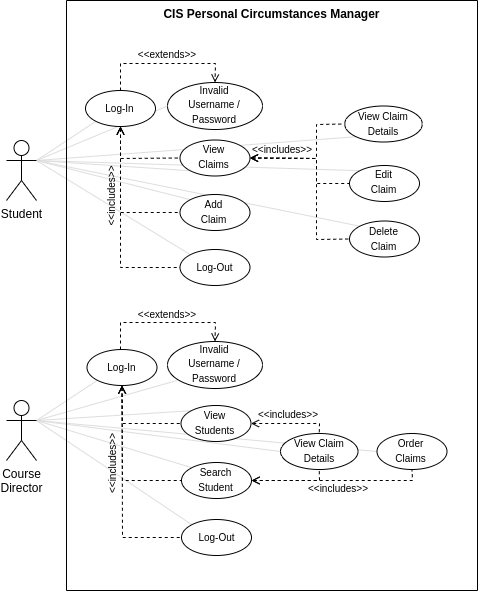
\includegraphics[width=14cm,height=18cm]{CS991_IMG/use_case.png}
	\end{center}

	\subsection{Use Case Descriptions}

	\begin{center}
		\scriptsize
	\begin{longtable}{p{3cm}|p{9cm}}
		\hline
		\hline
		\multicolumn{2}{c}{\textsc{Actor: Student}}\\
		\hline
		\hline
		\multicolumn{2}{c}{\textsc{Log-In}}\\
		\hline
		\textsc{Trigger} & A student wishes to log-in to their account.\\
		\textsc{Scenario} & A student wishes to view, edit, delete or add a personal cirumstances claim.\\
		\textsc{Precondition(s)} & A student must hold an account.\newline They must use their correct username and password to log-in.\\
		\textsc{Post Condition(s)} & A student has the ability to view, edit, delete or add a personal cirumstances claim, and log-out from within the system.\\
		\textsc{Main Path} & A student arrives at log-in page.\newline They select their account type: `student'.\newline They enter their username and password.\newline They select the submit button.\\
		\textsc{Alternative Path} & A student enters incorrect username/password.\newline They are prompted to complete the form again.\newline Or:\newline A student logs-out from within the system.\newline They must complete and submit the form again to log-back-in.\\
		\hline
		\multicolumn{2}{c}{\textsc{Invalid Username/Password}}\\
		\hline
		\textsc{Trigger} & A student enters the incorrect username/password combination.\\
		\textsc{Scenario} & A student has accidentally entered the wrong username/password.\newline A student has forgotten their username/password.\newline An unprepaired student is attempting to gain access to an account which is not theirs.\\
		\textsc{Precondition(s)} & A student must have a valid account (therefore, username/password).\newline They must enter either a valid existing username or password with an unmatching adjacent username/password.\\
		\textsc{Post Condition(s)} & A student is prompted to enter their log-in details again.\\
		\textsc{Main Path} & A student enters the wrong username/password relative to the account they're attempting to access at the username/password stage of the log-in protocol.\\
		\textsc{Alternative Path} & N/A\\
		\hline
		\multicolumn{2}{c}{\textsc{View Claims}}\\
		\hline
		\textsc{Trigger} & A student selects the `view claims option' from the student page header.\\
		\textsc{Scenario} & A student wishes to view their active (pending) claims.\newline A student wishes to view their expired (historically granted/denied) claims.\\
		\textsc{Precondition(s)} & A student must be logged-in.\\
		\textsc{Post Condition(s)} & A student can view all of their active and expired claims.\newline They have the option to edit or delete any active claim.\\
		\textsc{Main Path} & A student lands on this page after log-in.\\
		\textsc{Alternative Path} & They select the `view claims' option from the student page header. This is available from both the `view claims' and `add claim' pages.\\
		\hline
		\multicolumn{2}{c}{\textsc{View Claim Details}}\\
		\hline
		\textsc{Trigger} & A student selects the `view' option under the details heading from within a particular claim row.\\
		\textsc{Scenario} & A student wishes to view the additional text which they previously submitted under their claim details, when creating the claim.\\
		\textsc{Precondition(s)} & A student must be logged-in.\newline They must be on the `view claims' page.\\
		\textsc{Post Condition(s)} & A student can view the the additional text.\newline They can select the view option again to hide the additional text.\\
		\textsc{Main Path} & A student lands on the `view claims' page after log-in.\newline They select the `view' option under the details heading from within a particular claim row.\\
		\textsc{Alternative Path} & N/A\\
		\hline
		\multicolumn{2}{c}{\textsc{Edit Claim}}\\
		\hline
		\textsc{Trigger} & A student selects the `edit' option from within a particular claim row.\\
		\textsc{Scenario} & A student wishes to edit all possible details (title, start date, end date, details (description), attachments) of a previously submitted claim.\\
		\textsc{Precondition(s)} & A student must be logged-in.\newline They must be on the `view claims' page.\newline They must select an acitve claim to edit, the edit option is not available for expired claims.\\
		\textsc{Post Condition(s)} & A student is presented with a new page which resembles that of adding new claims where they can enter (change) the claim title, start date, end date, details (description), and attachments.\newline All of the claim's existing details are copied as placeholders to the input options.\newline They can use the submit button to submit the changes.\\
		\textsc{Main Path} & A student lands on the `view claims' page after log-in.\newline They select the `edit' option from within a particular claim row.\\
		\textsc{Alternative Path} & N/A\\
		\hline
		\multicolumn{2}{c}{\textsc{Delete Claim}}\\
		\hline
		\textsc{Trigger} & A student selects the `delete' option from within a particular claim row.\\
		\textsc{Scenario} & A student wishes to remove a previously submitted claim.\\
		\textsc{Precondition(s)} & A student must be logged in.\newline They must be on the `view claims' page.\newline They must select an acitve claim to delete, the delete option is not available for expired claims.\\
		\textsc{Post Condition(s)} & A claim and all of its attributes are removed from the system.\newline A student can no longer view this claim.\\
		\textsc{Main Path} & A student lands on the `view claims' page after log-in.\newline They select the `delete' option from within a particular claim row.\\
		\textsc{Alternative Path} & N/A\\
		\hline
		\multicolumn{2}{c}{\textsc{Add Claim}}\\
		\hline
		\textsc{Trigger} & A student selects the `add claim' option from the student page header.\\
		\textsc{Scenario} & A student wishes to add a new personal circumstances claim.\\
		\textsc{Precondition(s)} & A student must be logged in.\\
		\textsc{Post Condition(s)} & A student is presented with an input form where they can enter the claim title, start date, end date, details (description), and attachments of a new claim.\newline They can use the submit button to submit the new claim.\newline The new claim and all of its details will be available to view under `view claims' $\rightarrow$ `active claims'.\\
		\textsc{Main Path} & A student lands on the `view claims' page after log-in.\newline They select the `add claim' option from the student page header.\newline They land on the `add claim' page.\\
		\textsc{Alternative Path} & N/A\\
		\hline
		\multicolumn{2}{c}{\textsc{Log-Out}}\\
		\hline
		\textsc{Trigger} & A student wishes to log-out of their account.\\
		\textsc{Scenario} & A studdent wishes to terminate their browsing of their personal circumstance claims.\\
		\textsc{Precondition(s)} & A student must be logged-in to the system (meaning they are on the main site pages, not the log-in stages).\\
		\textsc{Post Condition(s)} & A student is returned to the log-in page (select account type step) and has the option to leave the site or to log-back-in.\\
		\textsc{Main Path} & A student is on any page of the main student system (i.e. not the login stages).\newline They select the `log-out' button on the header.\\
		\textsc{Alternative Path} & N/A\\
		\hline
		\hline
		\multicolumn{2}{c}{\textsc{Actor: Course Director}}\\
		\hline
		\hline
		\multicolumn{2}{c}{\textsc{Log-In}}\\
		\hline
		\textsc{Trigger} & A course director wishes to log-in to their account.\\
		\textsc{Scenario} & A course director wishes to view, edit, delete or add a personal cirumstances claim.\\
		\textsc{Precondition(s)} & A course director must hold an account.\newline They must use their correct username and password to log-in.\\
		\textsc{Post Condition(s)} & A course director has the ability view students (view claim details), search for a student (view claim details, order claims by date), and log-out from within the system.\\
		\textsc{Main Path} & A course director arrives at log-in page.\newline They select their account type: `course director'.\newline They enter their username and password.\newline They select the submit button.\\
		\textsc{Alternative Path} & A course director enters incorrect username/password.\newline They are prompted to complete the form again.\newline Or:\newline A course director logs-out from within the system.\newline They must complete and submit the form again to log-back-in.\\
		\hline
		\multicolumn{2}{c}{\textsc{Invalid Username/Password}}\\
		\hline
		\textsc{Trigger} & A course director enters the incorrect username/password combination.\\
		\textsc{Scenario} & A course director has accidentally entered the wrong username/password.\newline A course director has forgotten their username/password.\newline An unprepaired course director is attempting to gain access to an account which is not theirs.\\
		\textsc{Precondition(s)} & A course director must have a valid account (therefore, username/password).\newline They must enter either a valid existing username or password with an unmatching adjacent username/password.\\
		\textsc{Post Condition(s)} & A course director is prompted to enter their log-in details again.\\
		\textsc{Main Path} & A course director enters the wrong username/password relative to the account they're attempting to access at the username/password stage of the log-in protocol.\\
		\textsc{Alternative Path} & N/A\\
		\hline
		\multicolumn{2}{c}{\textsc{View Students}}\\
		\hline
		\textsc{Trigger} & A course director selects the `claims' option from the course director page header.\\
		\textsc{Scenario} & A course director wishes to view all active claims and all their associated details, by all registered students on the system.\\
		\textsc{Precondition(s)} & A course director must be logged-in.\\
		\textsc{Post Condition(s)} & A course director can view all students who have active claims.\\
		\textsc{Main Path} & A course director lands on this page after log-in.\\
		\textsc{Alternative Path} & They select the `claims' option from the course director page header. This is available from both the `claims' and `search' pages.\\
		\hline
		\multicolumn{2}{c}{\textsc{Search Student}}\\
		\hline
		\textsc{Trigger} & A course director selects the `search' option from the course director page header.\\
		\textsc{Scenario} & A course director wishes to search for a specific student (via their student ID) in order to view their active claims and all associated details.\\
		\textsc{Precondition(s)} & A course director must be logged-in.\\
		\textsc{Post Condition(s)} & A course director can display active claim details for any student of their choice.\\
		\textsc{Main Path} & A course director lands on the `claims' page after log-in.\newline They select the `search' option from the course director page header.\newline They input a student's ID.\newline They submit the request using the submit search button.\\
		\textsc{Alternative Path} & N/A\\
		\hline
		\multicolumn{2}{c}{\textsc{View Claim Details}}\\
		\hline
		\textsc{Trigger} & A course director selects `view' the option under the details heading from within a particular claim row.\\
		\textsc{Scenario} & A course director wishes to view the additional text which was submitted by students under their claim details, when creating the claim.\\
		\textsc{Precondition(s)} & A course director must be logged-in.\newline They must be on the `claims' page.\newline Or:\newline They must be on the `search', where results have been generated by student ID input and search submission.\\
		\textsc{Post Condition(s)} & A course director can view the the additional text.\newline They can select the view option again to hide the additional text.\\
		\textsc{Main Path} & A course director lands on the `claims' page after log-in.\newline They select the `view' option under the details heading from within a particular claim row.\\
		\textsc{Alternative Path} & A course director lands on the `claims' page after log-in.\newline They select the `search' option from the course director page header.\newline They search for a particular students claims using their student ID.\newline They select the `view option' under the details heading from within a particular claim row.\\
		\hline
		\multicolumn{2}{c}{\textsc{Order Claims}}\\
		\hline
		\textsc{Trigger} & A course director selects the an option from the order claims selection.\\
		\textsc{Scenario} & A course director wishes to order active claims for a specific result in descending order (newest first) (requirement), or ascending order (oldest first) (non-requirement).\\
		\textsc{Precondition(s)} & A course director must be loggen-in.\newline They must be on the `search', where results have been generated by student ID input and search submission.\\
		\textsc{Post Condition(s)} & A course director can display active claim details for any student of their choice, and choose to order the claims in an ascending or descending fashion.\\
		\textsc{Main Path} & A course director lands on the `claims' page after log-in.\newline They select the `search' option from the course director page header.\newline They input a student's ID.\newline They submit the request using the submit search button.\newline They select an option to sort the claims for the chosen student in ascending or descending order.\\
		\textsc{Alternative Path} & N/A\\
		\hline
		\multicolumn{2}{c}{\textsc{Log-Out}}\\
		\hline
		\textsc{Trigger} & To course director wishes to log-out of their account.\\
		\textsc{Scenario} & A course director wishes to terminate their browsing of students' personal circumstance claims.\\
		\textsc{Precondition(s)} & A course director must be logged-in to the system (meaning they are on the main site pages, not the log-in stages).\\
		\textsc{Post Condition(s)} & A course director is returned to the log-in page (select account type step) and has the option to leave the site or to log-back-in.\\
		\textsc{Main Path} & A course director is on any page of the main course director system (i.e. not the login stages).\newline They select the `log-out' button on the header.\\
		\textsc{Alternative Path} & N/A\\
		\hline
		\caption{Use Case Descriptions}
	\end{longtable}
	\end{center}
	
\newpage

\section{Medium Fidelity Prototype}

	This medium fidelity prototype developed for this project makes use of HTML, CSS and JavaScirpt in order to deliver a basically functioning user interface which responds in a way which would be reflected by the final application. However, it doesn't relay or fetch any database data. Data used in this example comes from basic HTML and JavaScript generations. Note that screenshots may be skewed / out of proportion as they are scaled to fit in equal rows and columns in a nice, neat \LaTeX\ table. For the sake of continuity and clarity, all use cases are presented here, not just three.

	\begin{center}
                \scriptsize
        \begin{longtable}{p{7cm}p{7cm}}
		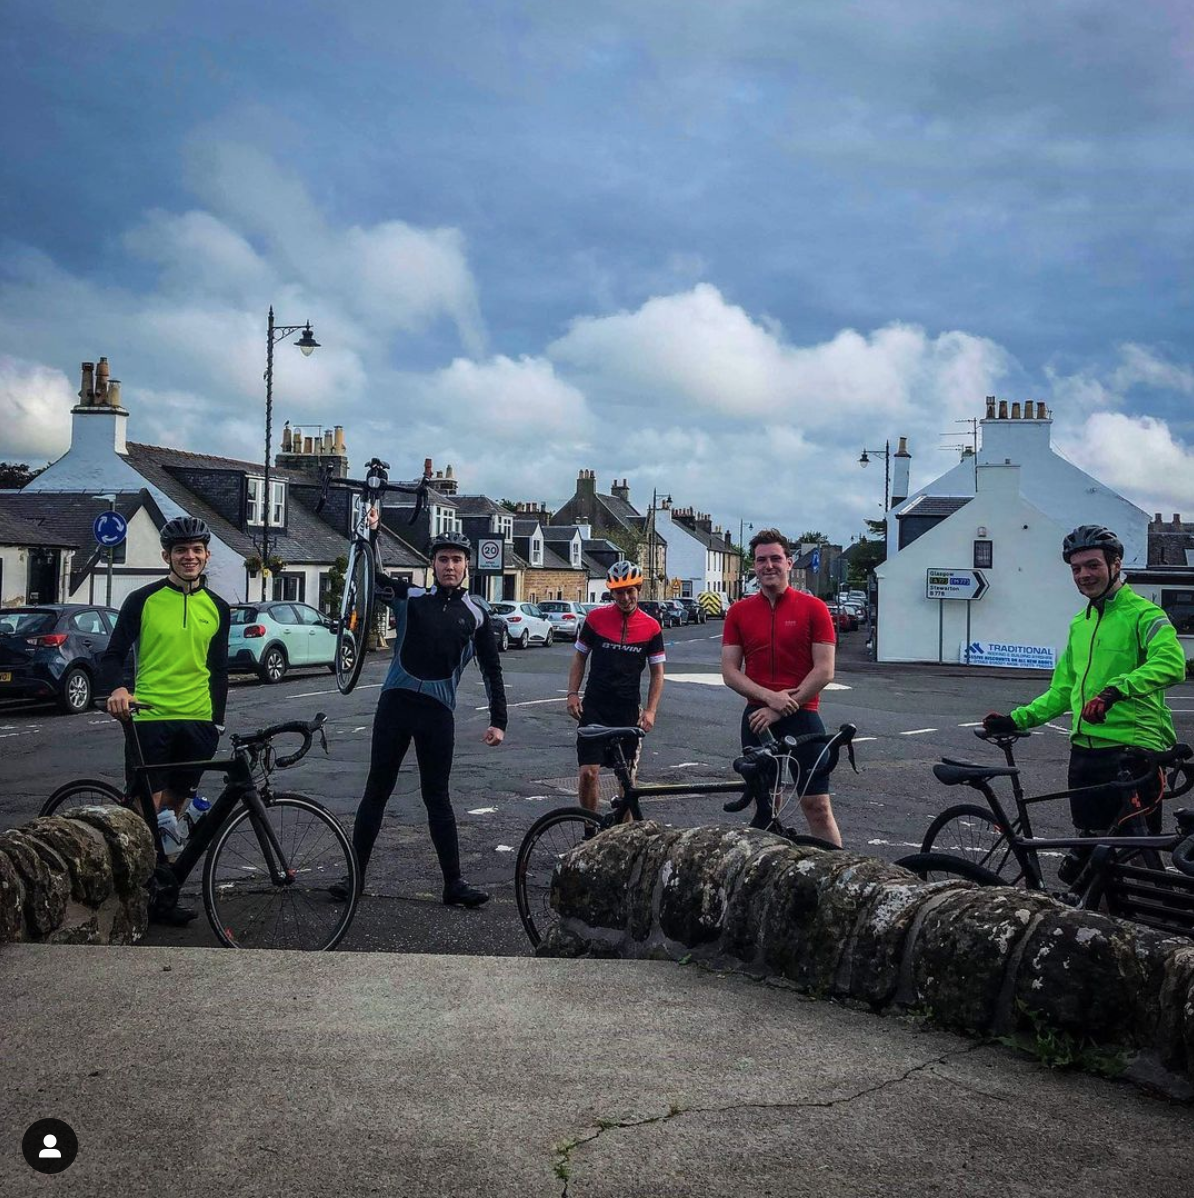
\includegraphics[width=5.5cm,height=9cm]{CS991_IMG/1.png} & 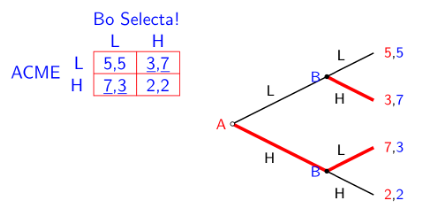
\includegraphics[width=5.5cm,height=9cm]{CS991_IMG/2.png}\\
		\textsc{Log-In (Student/Course Director)}\newline Basic login page. & \textsc{Log-In (Course Director)}\newline After selecting log-in as course director.\\
		
\includegraphics[width=6cm,height=9cm]{CS991_IMG/3.png} & 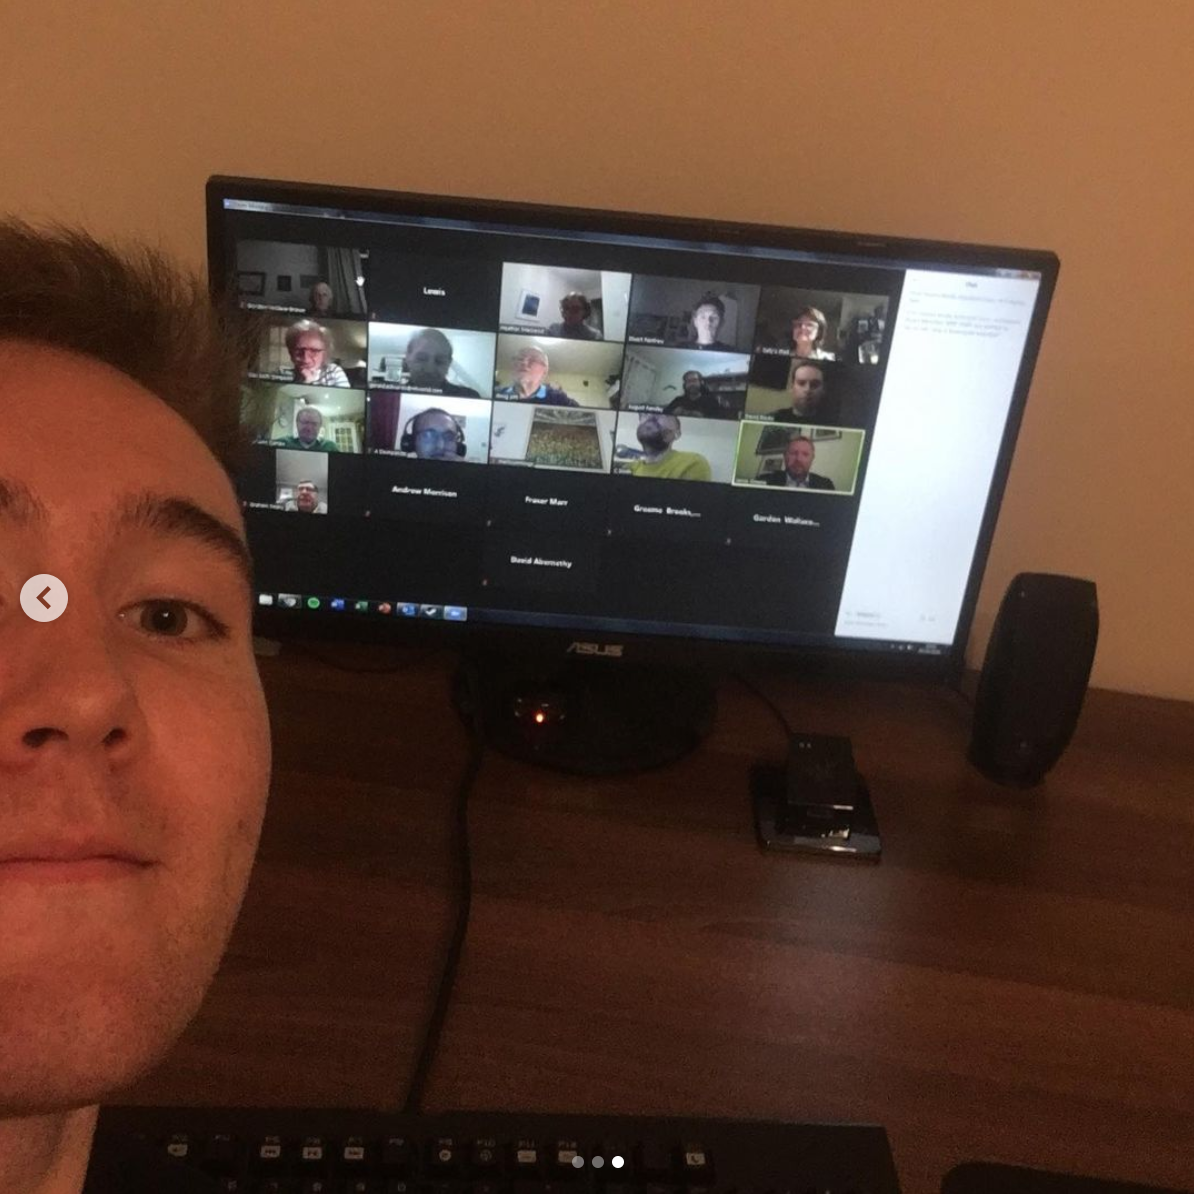
\includegraphics[width=6cm,height=9cm]{CS991_IMG/4.png}\\
		\textsc{Invalid Username/Password (Course Director)}\newline Incorrect or no details entered. & \textsc{Log-In (Student)}\newline After selecting log-in as student.\\
		& \\
		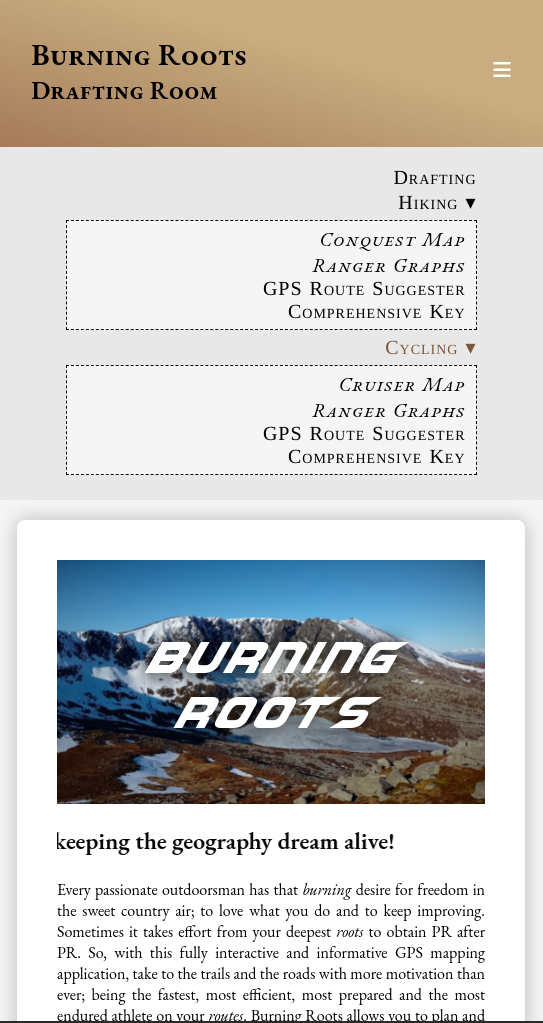
\includegraphics[width=6cm,height=9cm]{CS991_IMG/5.png} & \\
		\textsc{Invalid Username/Password (Student)}\newline Incorrect or no details entered. & \\ 
                \caption{Login Pages}
        \end{longtable}
        \end{center}

	\begin{center}
                \scriptsize
        \begin{longtable}{p{7cm}p{7cm}}
		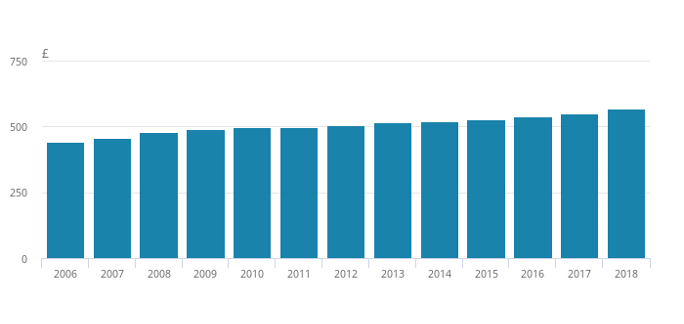
\includegraphics[width=5.5cm,height=9cm]{CS991_IMG/6.png} & 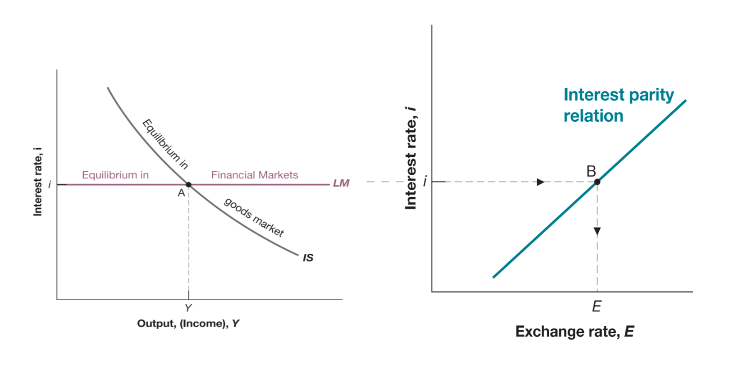
\includegraphics[width=5.5cm,height=9cm]{CS991_IMG/7.png}\\
		\textsc{View Students}\newline Select student page. & \textsc{View Students}\newline Student selected from drop-down, details appear for `Roger Federer'\\
		& \\
		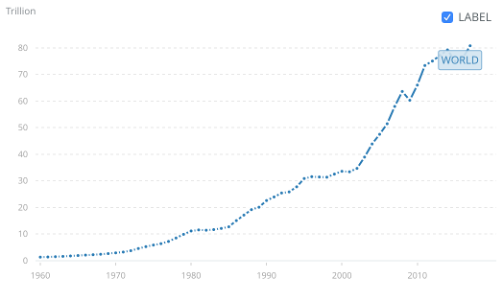
\includegraphics[width=5.5cm,height=9cm]{CS991_IMG/9.png} & 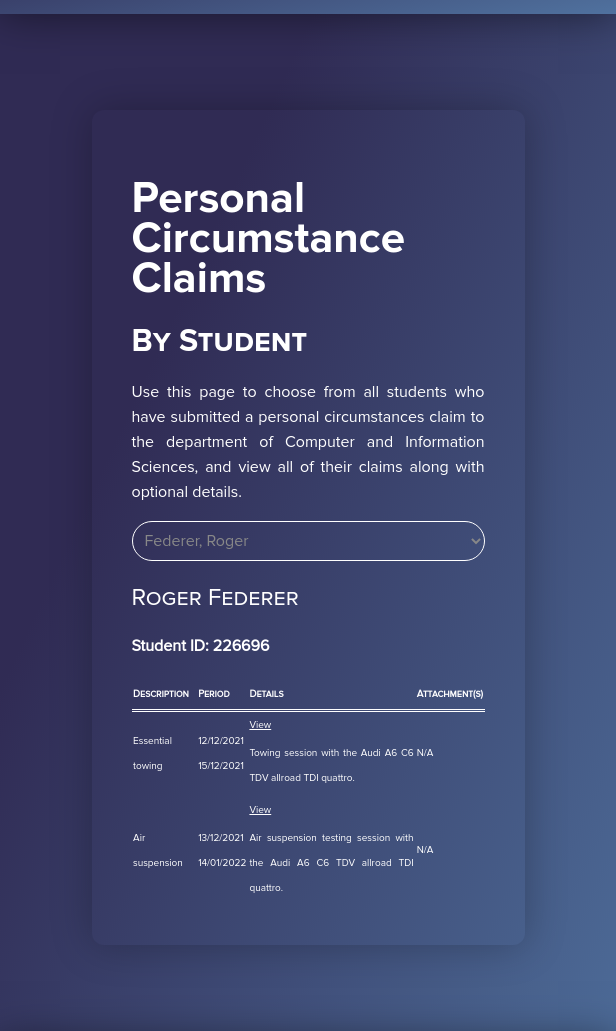
\includegraphics[width=5.5cm,height=9cm]{CS991_IMG/8.png}\\
		  \textsc{View Students}\newline Drop-down example. & \textsc{View Claim Details}\newline Selected option to view additional details of Roger's claims.\\
		 
\includegraphics[width=5.5cm,height=9cm]{CS991_IMG/10.png} & 
\includegraphics[width=5.5cm,height=9cm]{CS991_IMG/11.png}\\
		 \textsc{Search Student}\newline Search student page. & \textsc{Search Student}\newline Searched for `696226' and submitted using the search icon button. This resulted in `Rafael Nadal's claims being presented.\\
		 & \\
		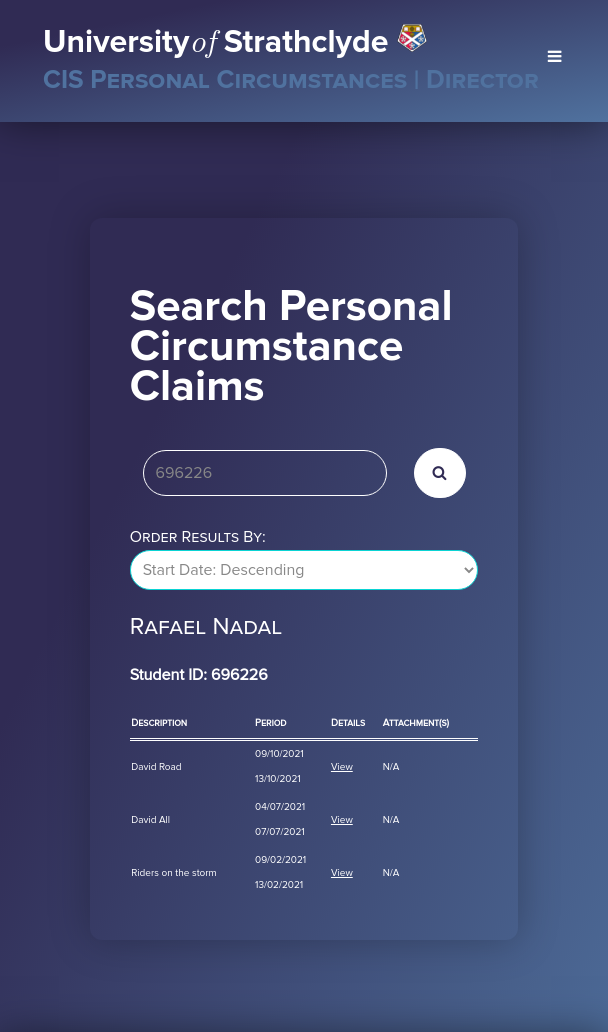
\includegraphics[width=5.5cm,height=9cm]{CS991_IMG/12.png} & 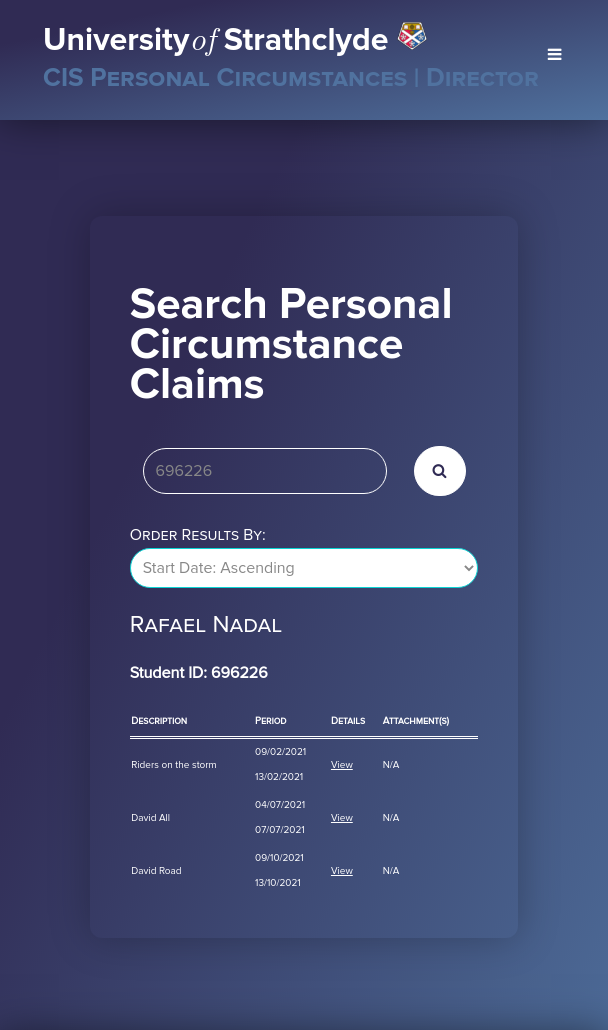
\includegraphics[width=5.5cm,height=9cm]{CS991_IMG/13.png}\\
		\textsc{Order Claims}\newline Sort: descending by start date (latest first), from drop-down. & \textsc{Order Claims}\newline Sort: ascending by start date (oldest first), from drop-down.\\
		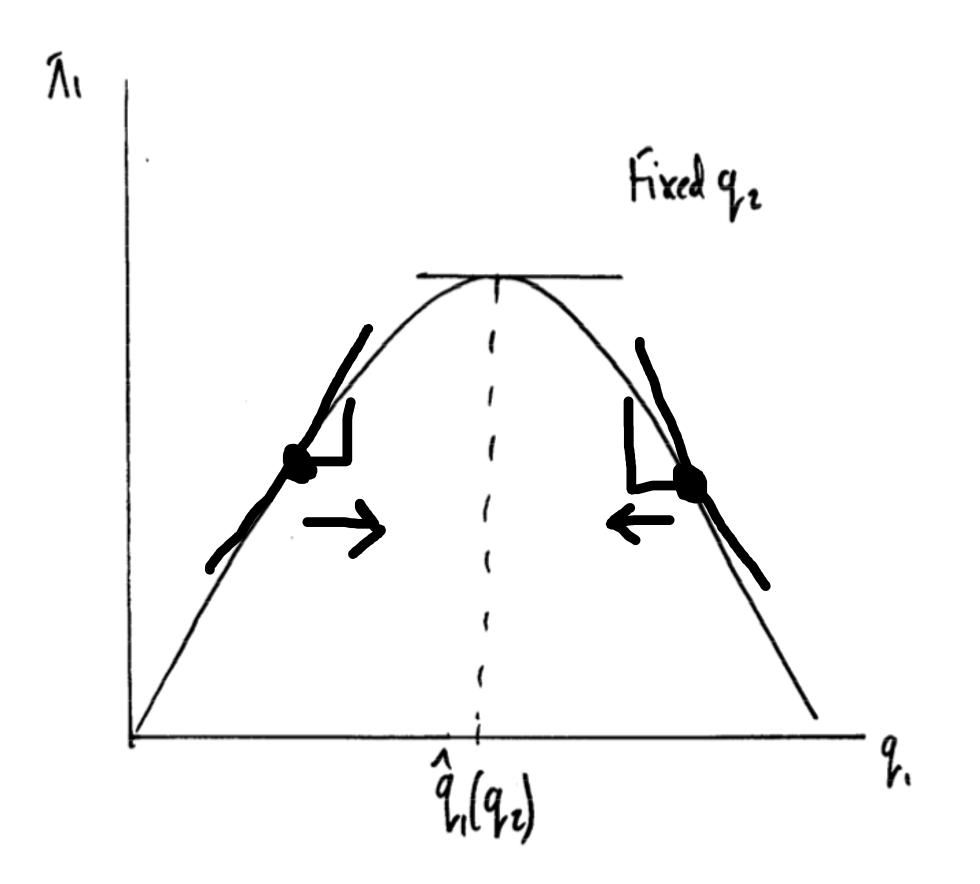
\includegraphics[width=5.5cm,height=9cm]{CS991_IMG/14.png} & \\
		Example of page select division under header from `hamburger' symbol. & \\
                \caption{Course Director Pages}
        \end{longtable}
        \end{center}

\newpage
	
	\begin{center}
                \scriptsize
        \begin{longtable}{p{7cm}p{7cm}}
		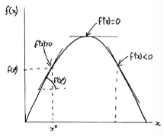
\includegraphics[width=5.5cm,height=9cm]{CS991_IMG/15.png} & 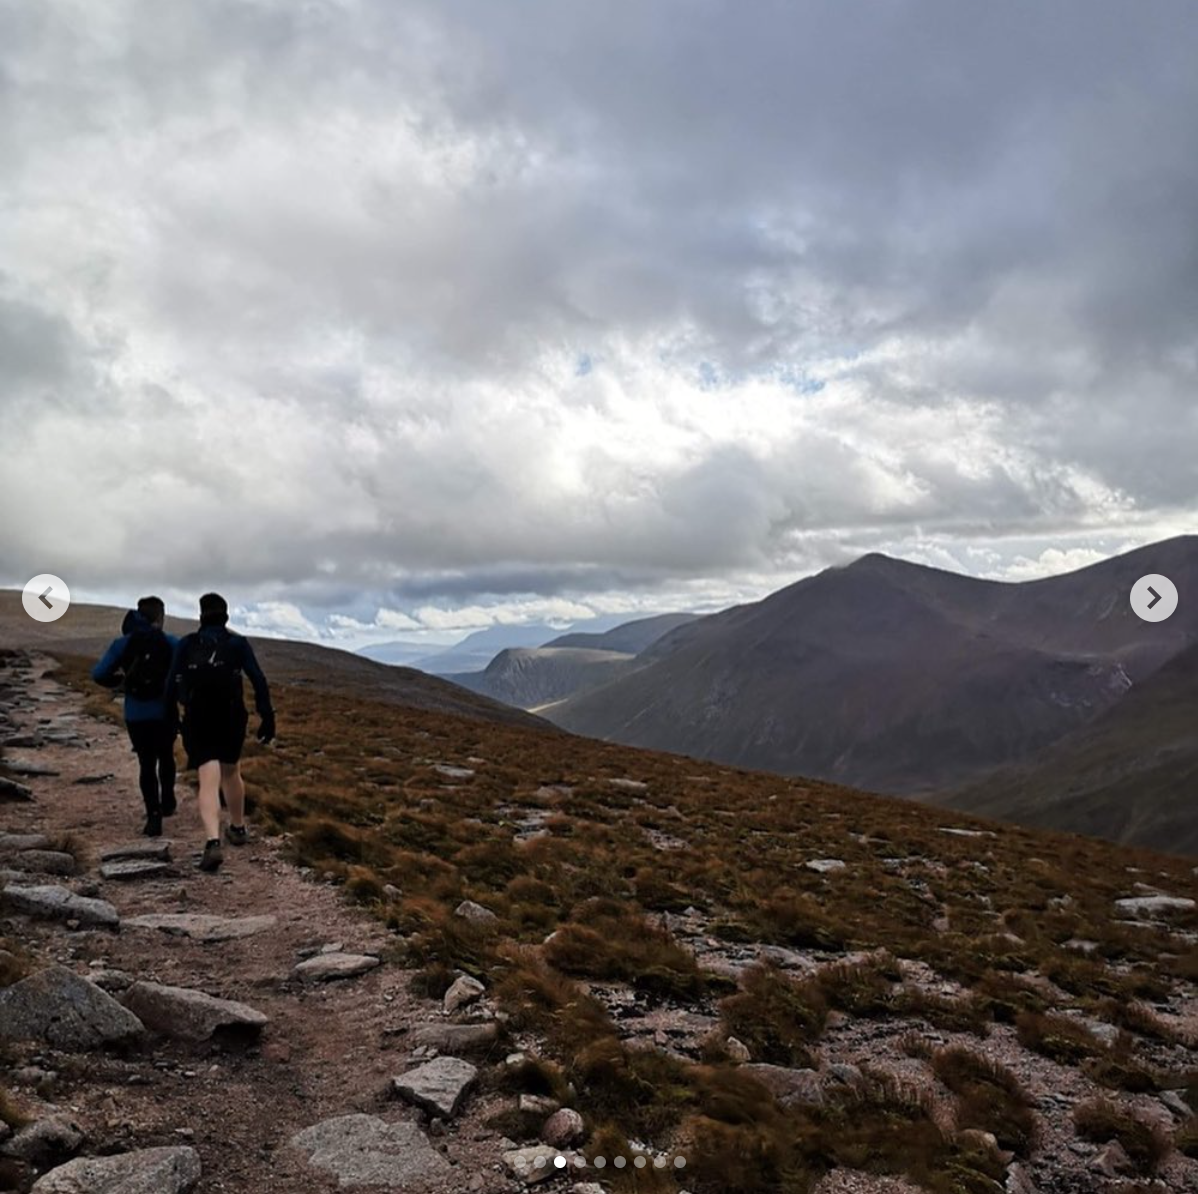
\includegraphics[width=5.5cm,height=9cm]{CS991_IMG/16.png}\\
		\textsc{View Claims}\newline View active and expired claims page. Options to delete and edit claims. & \textsc{Delete Claim}\newline Claim record missing after use of delete button.\\
		& \\
		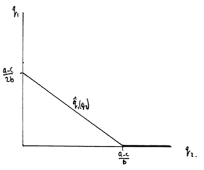
\includegraphics[width=5.5cm,height=9cm]{CS991_IMG/17.png} & 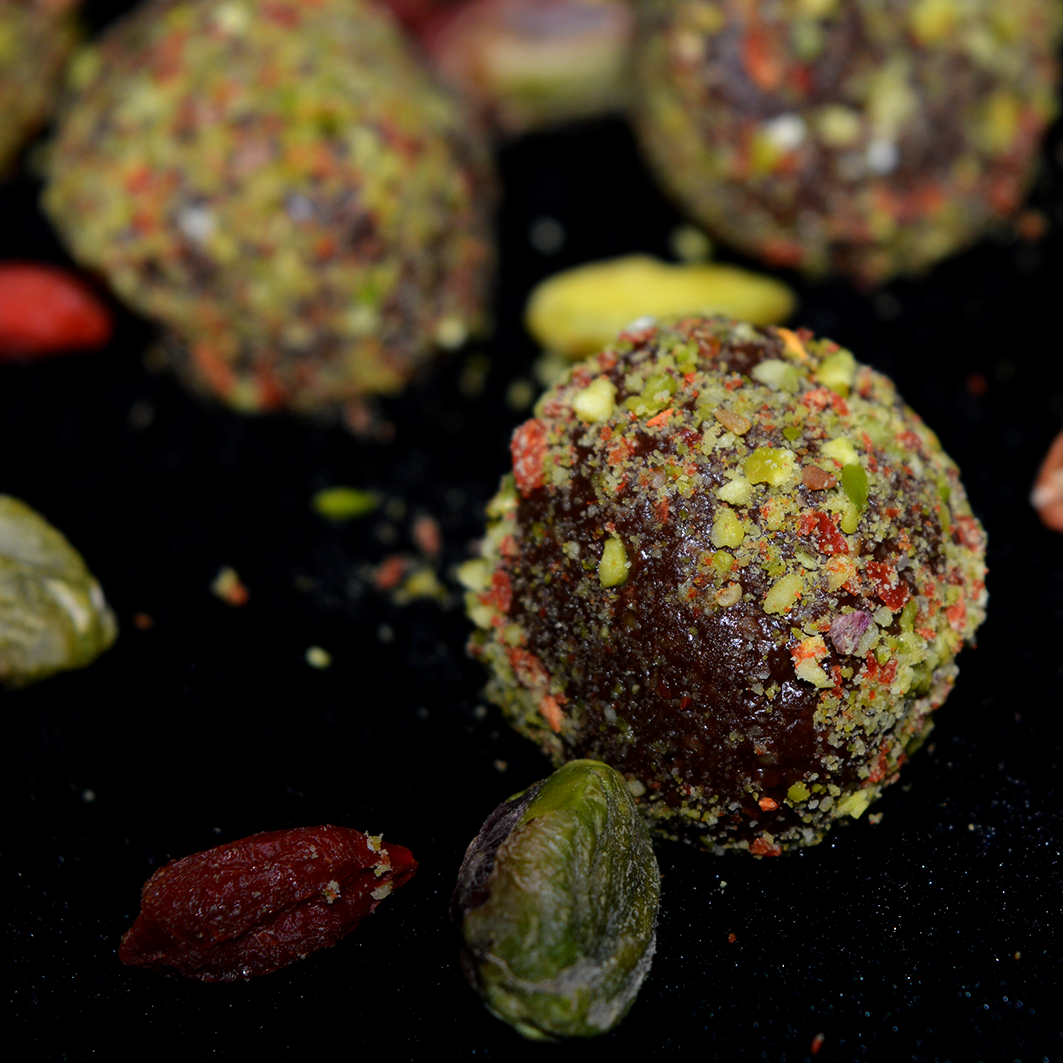
\includegraphics[width=5.5cm,height=9cm]{CS991_IMG/18.png}\\
		 \textsc{Edit Claim}\newline Edit claim page, using edit claim button from `Your Claims' page. Claim details copied as placeholders. Options to edit title, start date, end date, details, add file (input file), and submit. & \textsc{Add Claim}\newline Create new claim page. Options to input title, start date, end date, details, add file (input file), and submit.\\
                \caption{Student Pages}
        \end{longtable}
        \end{center}

\renewcommand\refname{Bibliography}

\begin{thebibliography}{9}

        \bibitem{a}
                Nielsen, J. (1994).
                \textsl{Heuristic Evaluation.}
		Usability Inspection Methods, John Wiley \& Sons

\end{thebibliography}

\end{document}
